\setcounter{chapter}{18}
\chapter{Effet photoélectrique}
\section{Le photon}
\subsection{Modèle onde - corpuscule}


\blocrouge{Rappels}{Le photon est une \trou{particule} (ou corpuscule) de masse \trou{nulle}. Le photon est la particule associée à un rayonnement électromagnétique. 

Jusqu'ici le rayonnement a été décrit par une \trou{onde}. Dans ce chapitre, il est décrit comme \trou{un flux} de photons.

Une onde électromagnétique se propageant dans le vide est décrit par une longueur d'onde $\lambda$ en m , une fréquence $\nu$ en \si{\per \second} et une vitesse de propagation $c=\SI{3.0e8}{\meter\per\second}$ 

On a alors $$\nu=\trou{\frac{c}{\lambda}}$$

}
\subsection{Energie d'un photon}

Chaque photon transporte une quantité d'énergie: E. Cette énergie est proportionnelle à la \trou{fréquence} du rayonnement (de l'onde) 

\blocrouge{Formule}{L'énergie d'un photon de fréquence $\nu$ vaut $$E=\trou{h\times \nu}$$
E en J ; $\nu$ la fréquence de l'onde en Hz ou \si{\per\second}\\ h=$\SI{6.63e-34}{\joule\per\second}$ est la constante de Planck 

}

\etiquette{Applications}
\begin{enumerate}
	\item Calculer la fréquence d'un photon violet $\lambda=\SI{400}{\nano\meter}$ et d'un photon rouge $\lambda=\SI{800}{\nano\meter}$ 
	\item Représenter sur un axe de longueur d'onde le domaine du visible et nommer les domaines voisins.
	\item Ajouter un axe correspondant à la fréquence des ondes électromagnétiques. Comment est-il orienté par rapport à l'axe en longueur d'onde ?
	\item Calculer en joules  l'énergie d'un photon violet et d'un photon rouge.
\end{enumerate}


\section{Effet photoélectrique}
\subsection{Description de l'expérience}
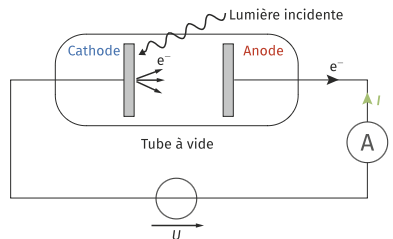
\includegraphics[width=.6\textwidth]{figures/effet_photoelectrique}\\
\url{https://phet.colorado.edu/sims/cheerpj/photoelectric/latest/photoelectric.html?simulation=photoelectric&locale=fr}\\
On éclaire en lumière monochromatique une plaque métallique. 

\blocrouge{Définition}{L'effet photoélectrique est le phénomène qui consiste en \trou{l'émission} d'électrons (courant électrique) par un matériau qui reçoit \trou{un rayonnement électromagnétique.}}

\subsection{Observations}
\begin{itemize}
	\item Pour certaines fréquences, on observe que la plaque émet \trou{des électrons}. 
	\item Il existe une fréquence \trou{seuil} en dessous de laquelle il ne se produit plus d'effet photoélectrique. 
	\item Même en augmentant l'intensité du rayonnement, si la fréquence est sous le seuil on \trou{n'observe pas }d'effet photoélectrique.
\end{itemize}

\subsection{Explications}

\begin{itemize}
	\item Les électrons de la plaque sont liés aux atomes par des forces \trou{attractives} (noyaux chargés +).
	\item En apportant une quantité d'énergie appelée \trou{travail d'extraction }(noté $W_{extraction}$) un électron est libéré de la plaque.
	\item Si l'énergie apportée par le photon est supérieure à $W_{extraction}$ alors l'excédant est \trou{emporté} par l'électron sous forme d'\trou{énergie cinétique}.
	\item L'énergie cinétique de l'électron lui permet de rejoindre l'anode et se traduit par un courant électrique que mesure \trou{l'ampèremètre}.
\end{itemize}

\blocrouge{Bilan énergétique}
{
 L'énergie d'un photon incident est utilisée pour extraire un électron et lui donner une énergie cinétique.\\
 Ecrivons la conservation de l'énergie:
 $$h\times \nu =\trou{W_{extraction}} + \trou{\frac{1}{2}m\times v^2} $$
}

\etiquette{Application}

Un photon d'énergie $Ec=\SI{5.03}{\eV}$ extrait un électron depuis une plaque de fer métallique. 
\begin{enumerate}
	\item Ecrire le bilan énergétique de cette situation.
	\item Calculer en joule, l'énergie cinétique maximale de l'électron arraché.
\end{enumerate}
On donne: $\SI{1}{\eV}=\SI{1.6e-19}{\J}$, pour un électron d'un atome de fer: $W_{extraction}=\SI{4.76}{\eV}$

\vspace{7cm}
\subsection{Ceci est une révolution !}

C'est l'interprétation de l'effet photoélectrique qui a permis de valider l'idée \trou{d'Einstein} selon laquelle l'interaction onde matière peut se décrire à l'aide d'une particule: le \trou{photon}. 

En effet, la description ondulatoire de la lumière ne peut rendre compte des résultats expérimentaux de l'expérience schématisée plus haut. Einstein obtient le prix \trou{Nobel} pour cette explication de l'effet photoélectrique par le photon. Cela marque le début de la \trou{mécanique quantique}.

%Lecture pour aller plus loin \url{https://query.libretexts.org/Francais/Physique_universitaire_III_-_Optique_et_physique_moderne_%28OpenStax%29/06%3A_Photons_et_ondes_de_matière/6.03%3A_Effet_photoélectrique}

\section{Absorption et Emission de photons}
\subsection{Absorption de photon}
\etiquette{Panneau photovoltaïque}

La surface d'un panneau photovoltaïque est constituée de cellules photovoltaïques. Chacune de ces cellules absorbe des photons et par effet photoélectrique produit un \trou{courant}.

Le rendement $\eta$ d'une cellule est le rapport entre la puissance électrique \trou{produite} et la puissance du rayonnement \trou{reçue}. $$\eta=\frac{\mathcal{P}_{elec}}{\mathcal{P}_{rayonnement}}$$

\etiquette{Capteur de lumière}

Dans un appareil photo (camera, téléphone, etc) le capteur est une surface tapissée de photodiodes. Chaque photodiode convertit la lumière reçue en courant électrique grâce à \trou{l'effet photoélectriqu}e.

\subsection{Emission de photon}
\etiquette{DEL Diode ElectroLuminescente}

Lorsque les électrons des atomes d'une DEL sont excités (par l'énergie électrique reçue) ils se désexcitent en émettant des photons. L'énergie de ces photons est liée au matériau qui constitue la DEL. 

\etiquetterouge{Exercices}

13, 14, 15 et 17 p 419
\\ \textbf{Préparer le bac} : 20 p 420
